\documentclass[12pt]{beamer}
\usepackage[utf8]{inputenc}
\usepackage[T1]{fontenc}
\usepackage{lmodern}
\usepackage[spanish, es-nodecimaldot, es-tabla]{babel}
\usepackage{amsmath}
\usepackage{amsfonts}
\usepackage{amssymb}
\usepackage{graphicx}
\usepackage{multicol}
% Insertar un gráfico standalone
\usepackage[mode=buildnew]{standalone}
\usetheme{Madrid}
% Paquete de Referenciación Natbib
\usepackage[numbers, round, sort, sectionbib]{natbib}
\renewcommand{\bibsection}{} % Para quitar la palabra bibliografía como título de esta sección o colocar otra. 
\setcitestyle{square}
\bibliographystyle{vancouver}

\begin{document}
	\author[Daniel Parra]{Daniel S. Parra G.}
	\title[IVM en el tratamiento de infección]{Ivermectina en el tratamiento de infección por SARS-CoV-2}
	\subtitle{Simulación PKPD-VK}
	%\logo{}
	%\institute[]{Universidad Nacional de Colombia}
	\date{\today}
	%\subject{}
	%\setbeamercovered{transparent}
	%\setbeamertemplate{navigation symbols}{}
	\begin{frame}[plain]
		\maketitle
	\end{frame}
	
	\begin{frame}{Contenido}
		\tableofcontents[currentsection]
	\end{frame}
	
	\section{Introducción}
	\begin{frame}{Introducción}
		No es factible la utilización de la ivermectina en el tratamiento del COVID-19 aunque exista evidencia anecdótica, testimonios, o estudios observacionales que muestren una utilidad.
	\end{frame}
	
	\begin{frame}{Introducción}
		\begin{itemize}
			\small\setlength\itemsep{1.5em}
			\item En marzo de 2020 se publicó un estudio que mostraba actividad \textit{in vitro} de ivermectina frente al SARS-CoV-2 (\textit{Caly et al} \cite{Caly2020}). \\
			
			\item  En el resumen del estudio se mostraba una reducción de 5000 veces en RNA viral de SARS-CoV-2 con ivermectina en 48 horas, por lo cual los autores decían que esto merecía una mejor investigación por posibles beneficios en seres humanos. \\
			
			\item Según los autores el efecto podría deberse a la inhibición en la unión de una proteína del SARS-Cov-2 con el complejo de proteínas de importe $\mathrm{IMP}\text{-}\alpha/\beta_{1}$. Lo que resultaba en una disminución del transporte nuclear de la proteína de SARS-CoV-2, y esto podría permitir una mejor respuesta intracelular del hospedero. 
		\end{itemize}
	\end{frame}

	\begin{frame}{Introducción}
		\begin{multicols}{2}
			
			\scriptsize 
			A la derecha, se muestra una figura del estudio \cite{Caly2020}, según la cual se muestra una ``potente'' actividad de la ivermectina. \\
			\vspace{4em}\scriptsize 
			\textbf{Tomado de}: Caly L, Druce JD, Catton MG, et al. The FDA-approved Drug Ivermectin inhibits the replication of SARS-CoV-2 in vitro. \textit{Antiviral Res} 2020; 104787. 
			\columnbreak
			
			\begin{figure}
				\centering
				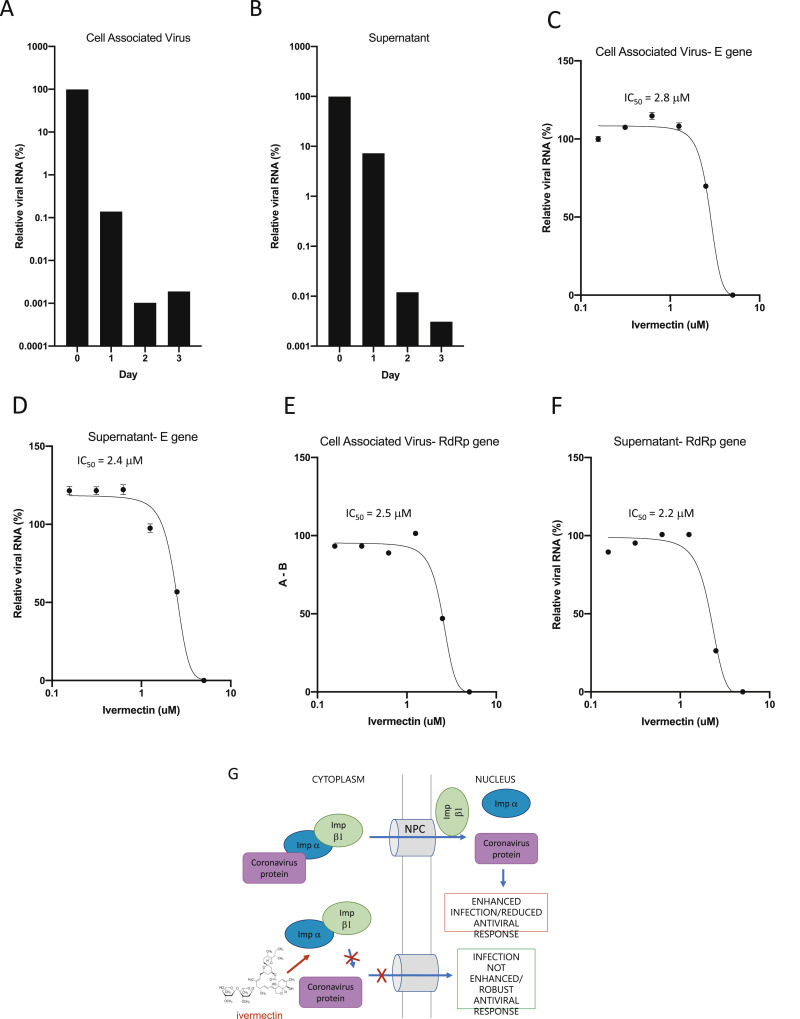
\includegraphics[width=1\columnwidth]{figs/Caly_Extracted_Image}
				\label{fig:calyextractedimage}
			\end{figure}	
		\end{multicols}
	\end{frame}

	\begin{frame}{Introducción}
		\small De inmediato, se despertó un gran interés mediático por un tratarse de un posible ``tratamiento''. Con titulares mostrando sus ``beneficios en menos de 72 horas'', y esto claramente despertó el interés del público:

		\begin{figure}
			\centering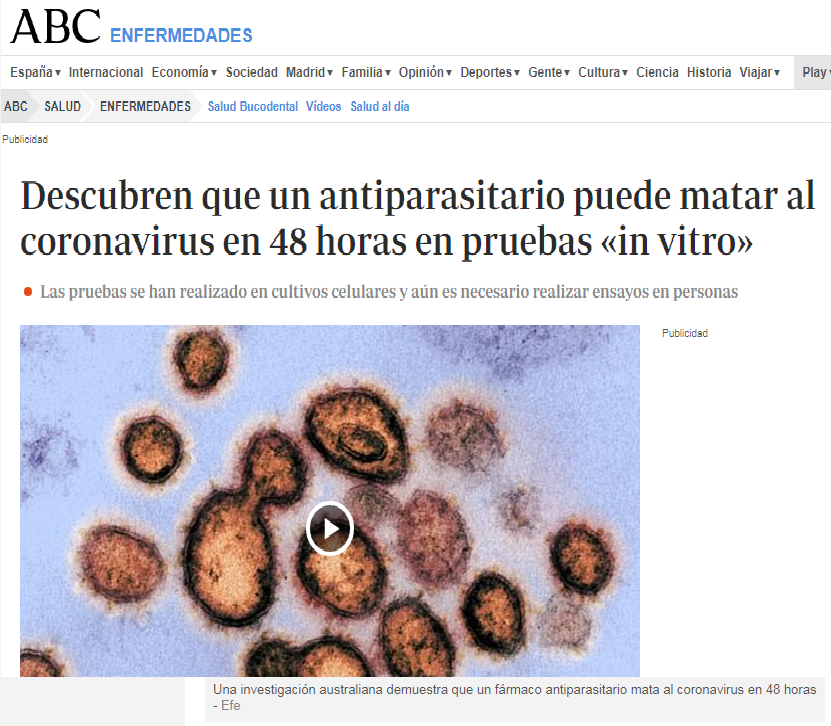
\includegraphics[width=0.7\linewidth]{figs/titular_1}
			\label{fig:titular1}
		\end{figure}
	\end{frame}

	\begin{frame}{Resultados Búsquedas en Google}		
		\scriptsize El interés de público se puede medir de forma aproximada con la cantidad de búsquedas del término en buscadores web. 
		\begin{figure}
			\centering
			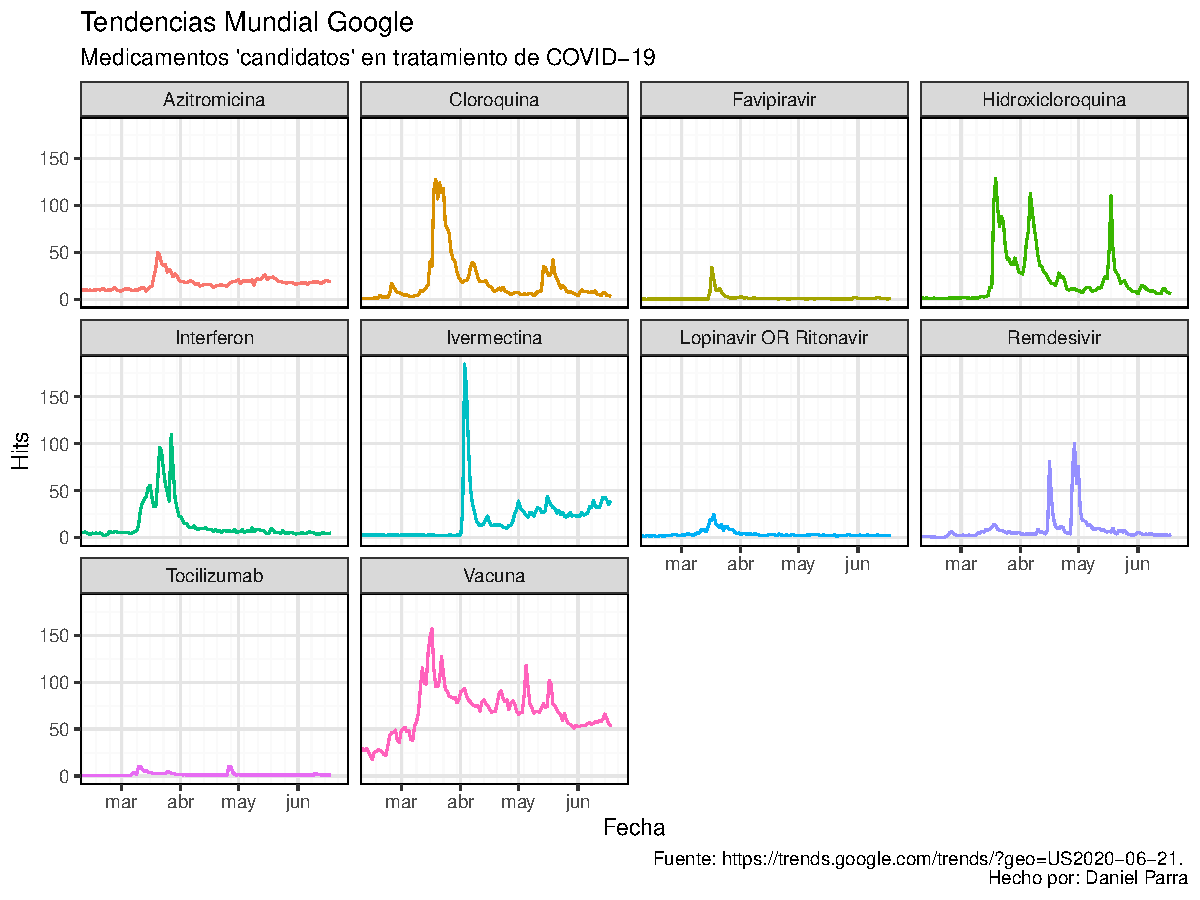
\includegraphics[width=0.8\linewidth]{../../6_Google_Trends/figures/G2_2020-06-21}
			\label{fig:g1col2020-06-21}
		\end{figure}
	\end{frame}

	\section{Farmacocinética}
	\begin{frame}{Farmacocinética}
		\small
		\begin{itemize}
	 		\item El argumento farmacocinético respecto a la factibilidad de su uso es importante, y puede ser uno de los principales causantes para que gran parte de la comunidad científica no haya explorado su uso aplicado en seres humanos con esta indicación. \\
			
			\item En el estudio se reporta el valor de $\mathrm{IC_{50}}$ en el orden de $2~\mu\mathrm{M}$, que es una concentración muy alta (si tenemos en cuenta una masa molecular de $875.1~\mathrm{g/mol}$). \\
						
			\item Una dosis habitual es 0.15 mg/kg (10.5mg en individuo de 70kg) cada \textbf{12 meses} en oncocercosis (ceguera del rio).
		\end{itemize}
	\end{frame}
	
	\begin{frame}{Farmacocinética}
		\scriptsize
		En respuesta al reporte de \textit{Caly et al.} se escribió correspondencia mostrando que es imposible alcanzar las concentraciones de IVM \textit{in vitro} en seres humanos con los regímenes de dosificación conocidos \citep{Rayner2020}. 
		\begin{figure}
			\centering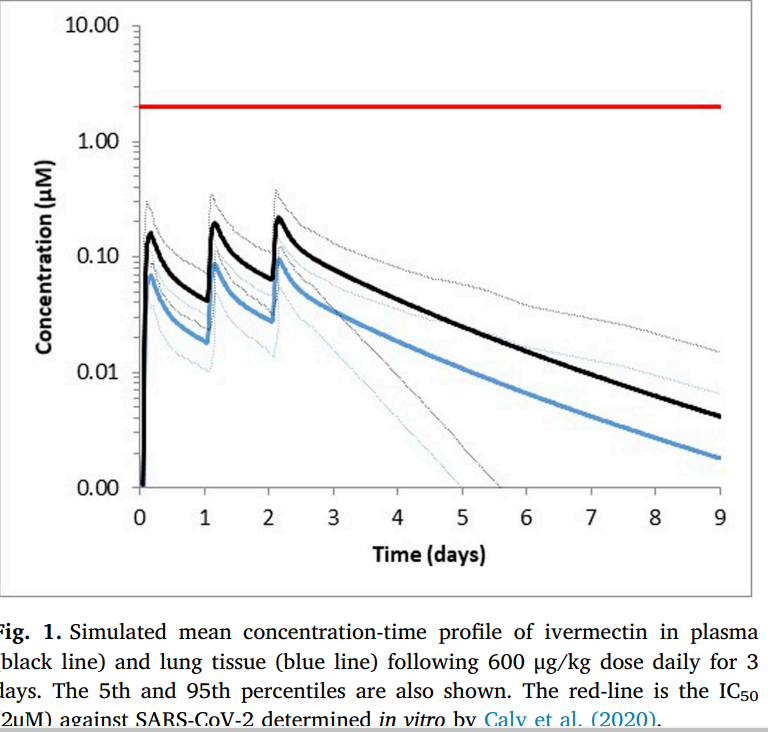
\includegraphics[width=0.5\linewidth]{figs/ivermectin_profile}
		\end{figure}
	\end{frame}
	
	\begin{frame}{Experimento mental}
		\scriptsize
		Que tal si simulamos una \textbf{dosis} que alcance ese valor para inhibir la replicación del virus. Se propone un régimen con algunos modelos de farmacocinética poblacional reportados en literatura: 
		\begin{enumerate}
			\setlength\itemsep{1.5em}
			\item Duthaler U, Suenderhauf C, Karlsson MO, et al. Population pharmacokinetics of oral ivermectin in venous plasma and dried blood spots in healthy volunteers. \textit{Br J Clin Pharmacol} 2019; 85: 626–633. \cite{Duthaler2019}
			\item El-Tahtawy A, Glue P, Andrews EN, et al. The effect of azithromycin on ivermectin pharmacokinetics - A population pharmacokinetic model analysis. \textit{PLoS Negl Trop Dis}; 2. \cite{El-Tahtawy2008}
			\item Smit MR, Ochomo EO, Waterhouse D, et al. Pharmacokinetics-Pharmacodynamics of High-Dose Ivermectin with Dihydroartemisinin-Piperaquine on Mosquitocidal Activity and QT-Prolongation (IVERMAL). \textit{Clin Pharmacol Ther} 2019; 105: 388–401. \cite{Smit2019}
			\item Duthaler U, Leisegang R, Karlsson MO, et al. The effect of food on the pharmacokinetics of oral ivermectin. \textit{J Antimicrob Chemother} 2020; 75: 438–440. \cite{Duthaler2020}
		\end{enumerate}
	\end{frame}

	\begin{frame}
		\frametitle[Experimento mental]{Simulación PK de ivermectina}
		\begin{figure}[t]
			\centering
			%\caption{}
			\label{fig:pk2opcional8}
			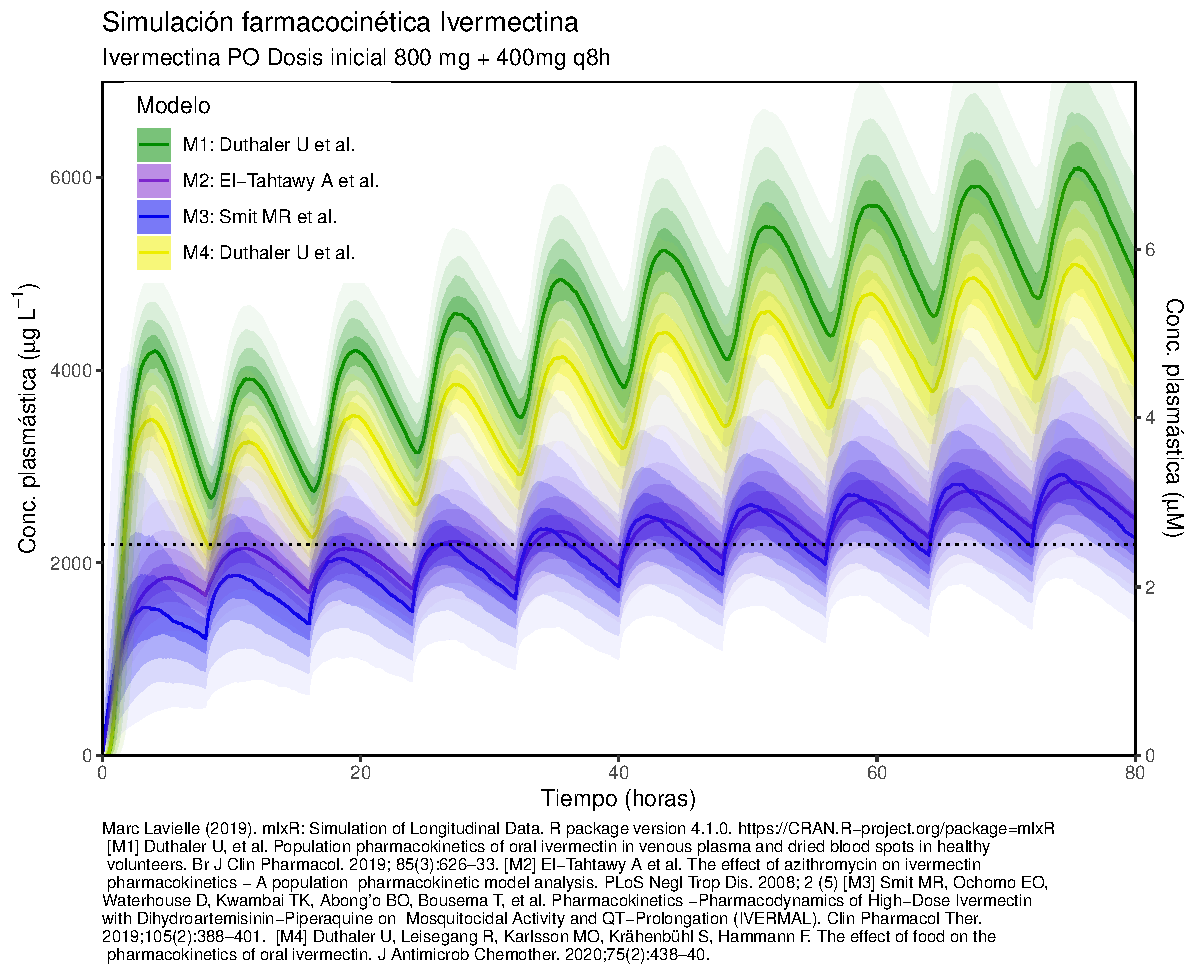
\includegraphics[width=0.8\linewidth]{../modelo_pkpd/PK2_opcional8}
		\end{figure}
	\end{frame}

	\begin{frame}
		\frametitle[Experimento mental]{Simulación PK de IVM}
		\small
		Se tendría un régimen de 800mg (dosis de carga) + 400mg q8h, y esto está muy encima de los recomendado en seres humanos. Si tomamos una solución peroral de IVM de 6mg/mL en frasco por 30mL, esto equivaldría a 6.66 frascos diarios!!!, algo así como 200mL diarios de solución. \\
		\vspace{4em}
		\textbf{Supuesto}: la farmacocinética sigue siendo lineal con estas dosis (improbable), se da la posibilidad que estas concentraciones no puedan ser alcanzadas \textit{in vivo}.
	\end{frame}
	
	\section{Farmacodinamia}
	
	\begin{frame}
		\frametitle[]{Experimento mental}\framesubtitle{Farmacodinamia}
		Que tal si evaluamos la farmacodinamia, ya con el efecto que tendrían estas concentraciones. \\
		\vspace{2em}
		Si consideramos una dosis base de 12mg q8h (que ya es bastante alta p.ej. en escabiosis (piojos) se utilizan dos dosis de $200~\mu\mathrm{g/kg/dosis}$ separadas por una semana), y la multiplicamos por 2, 5, 10, y 15 veces se tienen los perfiles PK mostrados en la diapositiva siguiente. 
	\end{frame}

	\begin{frame}	
		\frametitle{Farmacocinética}			
		\begin{figure}
			\centering
			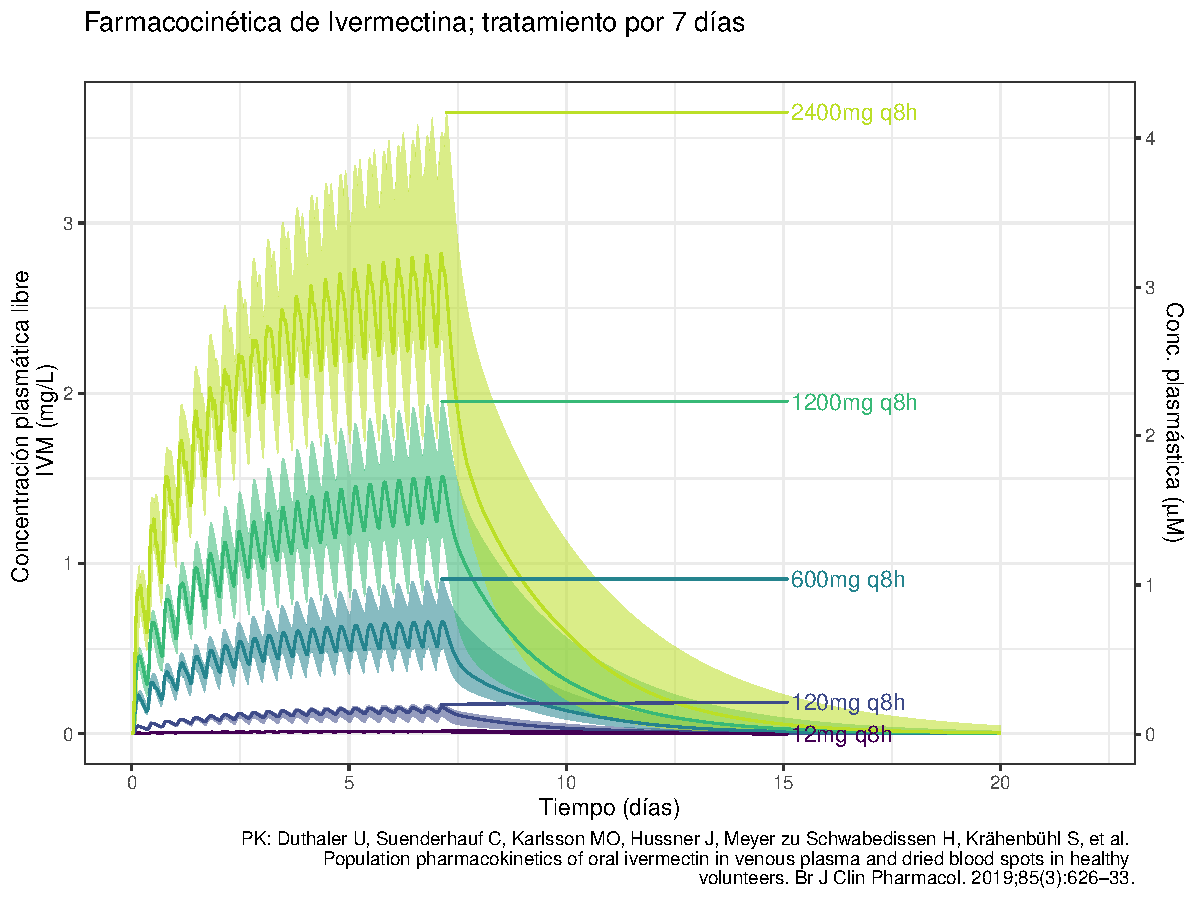
\includegraphics[width=0.9\linewidth]{../modelo_PD_2/figuras/G1}
			%\caption{}
			\label{fig:g1}
		\end{figure}
	\end{frame}
	
	\begin{frame}
		\frametitle{Modelamiento PD ivermectina}
		\begin{figure}
			\centering
			\includegraphics[width=0.8\linewidth]{../modelo_PD/modelo_ivermectina}
			%\caption{}
			\label{fig:modeloivermectina}
		\end{figure}
	\end{frame}
	
	\begin{frame}	
		\frametitle{Farmacodinámica}		
		\begin{figure}
			\centering
			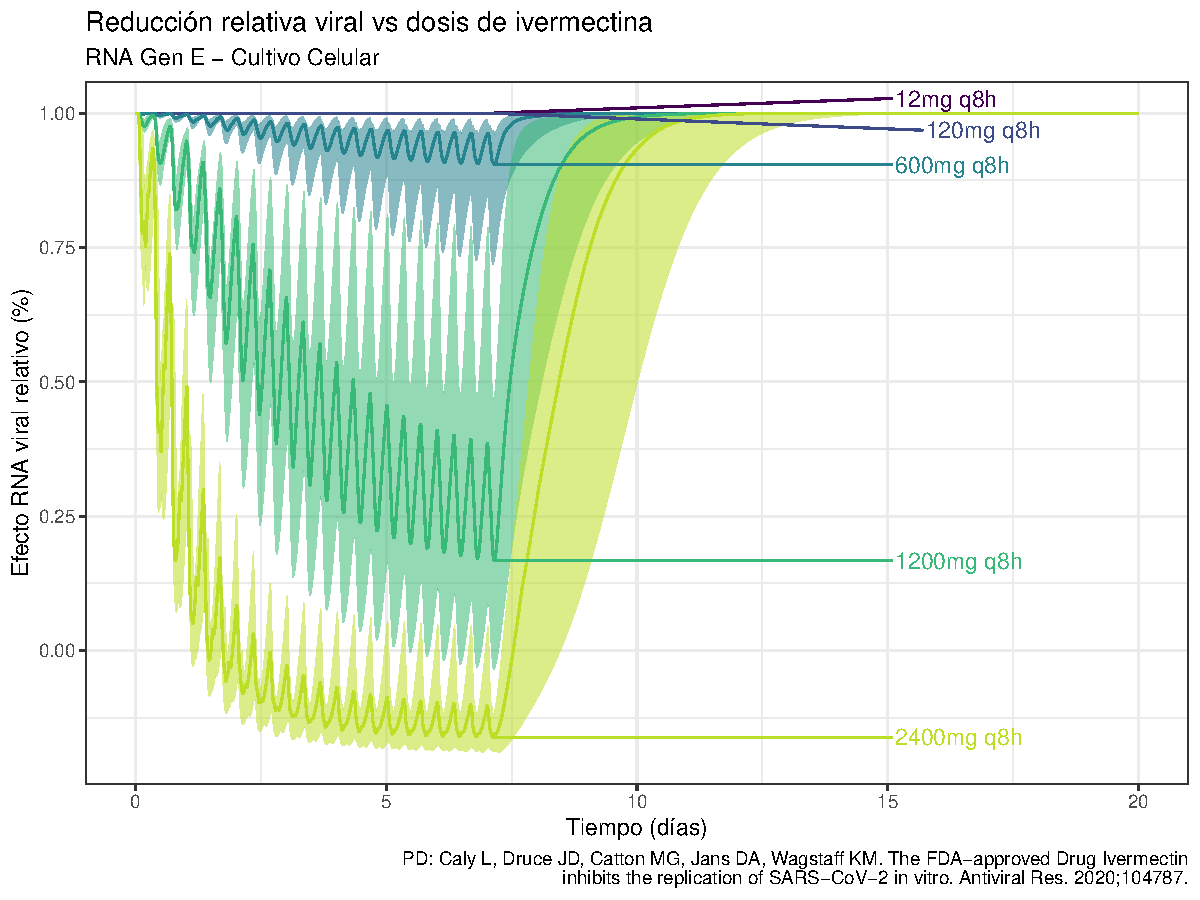
\includegraphics[width=0.9\linewidth]{../modelo_PD_2/figuras/G2}
			%\caption{}
			\label{fig:g1}
		\end{figure}
	\end{frame}
	
	\section{Cinética viral}
	
	\begin{frame}
		\frametitle{Modelo combinado}
		\centering
		\includestandalone[width=1\textwidth]{tikz/imagen_tikz}
		
		\bigskip
		\parbox[b]{1.0\textwidth}{\tiny \textbf{Modelo PK}: Duthaler U, Suenderhauf C, Karlsson MO, et al. Population pharmacokinetics of oral ivermectin in venous plasma and dried blood spots in healthy volunteers. Br J Clin Pharmacol 2019; 85: 626–633. \\
			\textbf{Modelo PD}: Caly L, Druce JD, Catton MG, et al. The FDA-approved Drug Ivermectin inhibits the replication of SARS-CoV-2 in vitro. Antiviral Res 2020; 104787.\\
			\textbf{Modelo VK}: Kim KS, Ejima K, Ito Y, et al. Modelling SARS-CoV-2 Dynamics: Implications for Therapy. medRxiv 2020; 2020.03.23.20040493.}
	\end{frame}
	
	\begin{frame}	
		\frametitle{Cinética viral (1)}		
		\begin{figure}
			\centering
			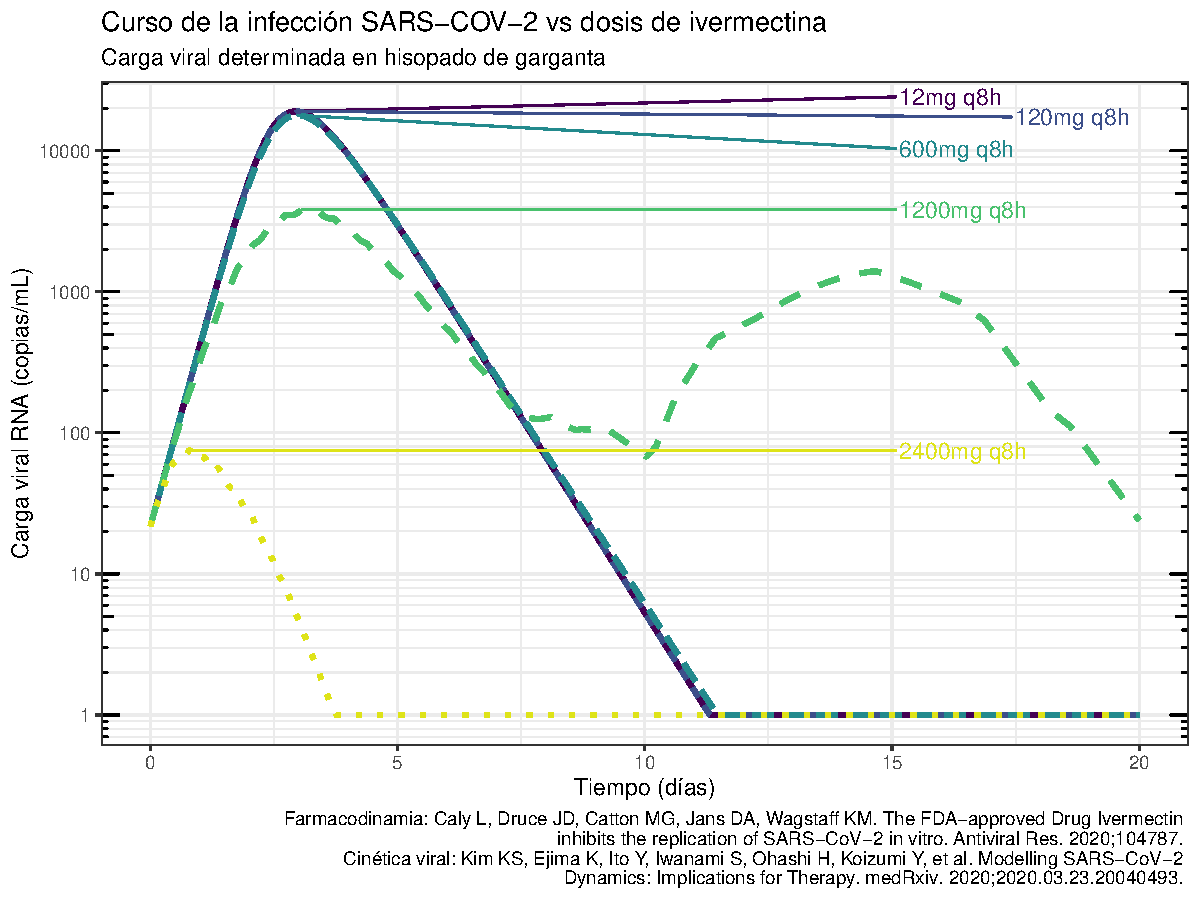
\includegraphics[width=0.9\linewidth]{../modelo_PD_2/figuras/G3}
			%\caption{}
			\label{fig:g1}
		\end{figure}
	\end{frame}

	\begin{frame}	
		\frametitle{Cinética viral (2)}	
		\begin{figure}
			\centering
			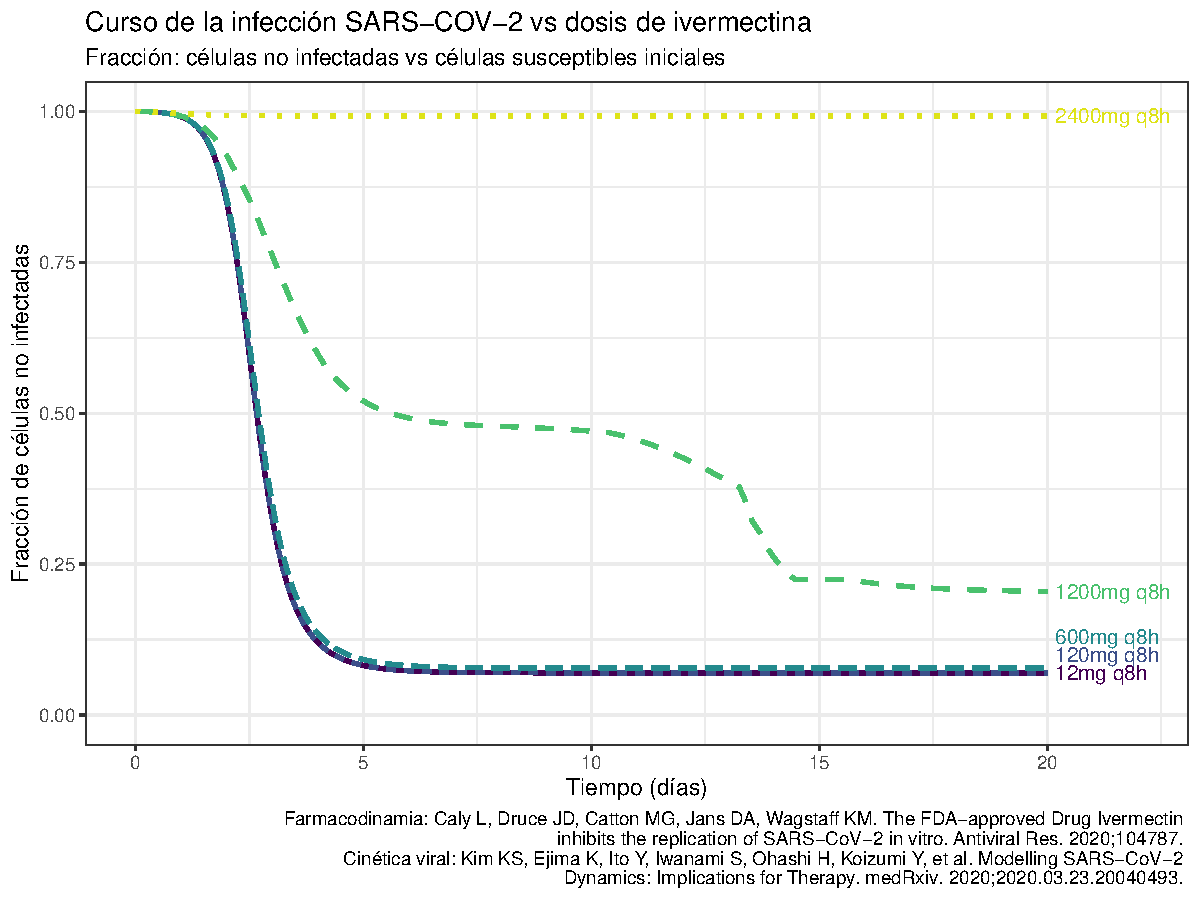
\includegraphics[width=0.9\linewidth]{../modelo_PD_2/figuras/G4}
			%\caption{}
			\label{fig:g1}
		\end{figure}
	\end{frame}
	
	\begin{frame}
		\frametitle[Mapa IVM]{Treemap Ivermectina}
		\begin{figure}[t]
			\centering
			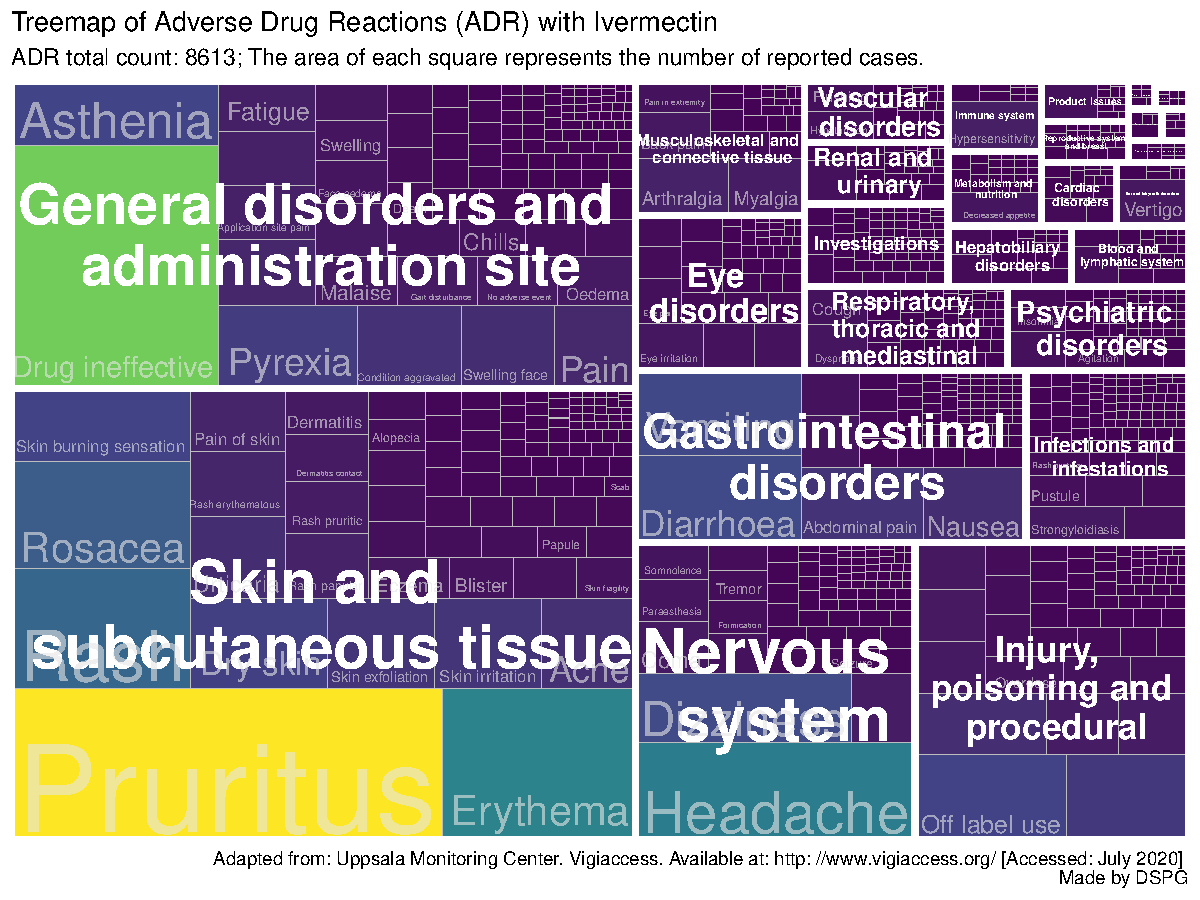
\includegraphics[width=0.8\linewidth]{../seguridad_IVM/Heat_Map_IVM}
%			\caption{\tiny Mapa de árbol de Reacciones Adversas de Medicamentos (RAM) de ivermectina.}
			\label{fig:heatmapivm}
		\end{figure}
	\end{frame}

	\begin{frame}{Referencias}
		\bibliography{referencias}
	\end{frame}
\end{document}